%!TEX root = main.tex
\vspace{-.8cm}
\section{Methodology} % (fold)
\label{sec:model}

\begin{wrapfigure}[19]{r}{0.5\textwidth}
%\begin{figure}[H]
	\setlength{\abovecaptionskip}{-0.1em}
	\setlength{\belowcaptionskip}{-1em}
	\pgfdeclarelayer{background}
	\pgfdeclarelayer{foreground}
	\pgfsetlayers{background,main,foreground}
	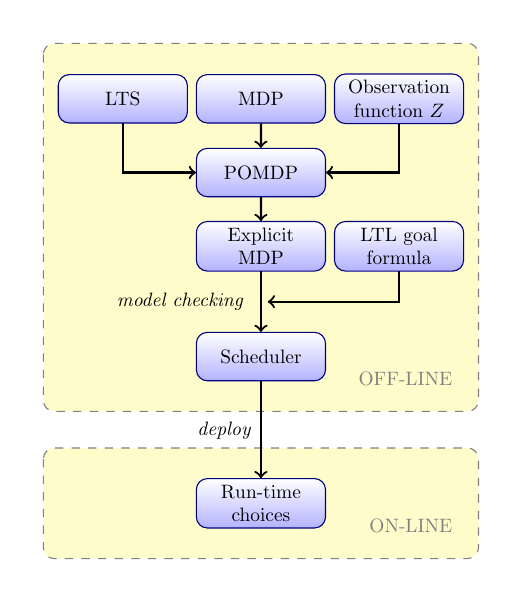
\begin{tikzpicture} [
	   auto, scale=0.7, every node/.style={scale=0.7},
	   block/.style    = { rectangle, top color=white, bottom color=blue!30, 
	                            draw=blue!50!black!100, text width=6em, text centered, rounded corners, minimum height=2.5em },
	   line/.style     = { draw,thick,->,minimum height=1em },
	 ]
	  % Define nodes in a matrix
	  \matrix [column sep=1mm, row sep=3mm] {
	  	\node (pos1){}; &&&& \\
		&\node [block] (phase1){LTS}; & \node [block] (phase2){MDP}; & \node [block] (phase3){Observation function $Z$}; & \\
		&& \node [block] (phase4){POMDP}; && \\
		&& \node [block] (phase5){Explicit MDP}; & \node [block] (phase6) {LTL goal formula}; & \\
		&& \node (null2) {}; && \\
		&& \node [block] (phase7){Scheduler}; && \\
		&&&& \node (pos2){}; \\
		\node (pos3){}; && \node (null3){};&& \\
		&& \node [block] (phase8){Run-time choices}; && \\
		&&&& \node (pos4){}; \\
	 };

	 \node (mc) at (null2)[left=5pt] {\textit{model checking}};
	 \node (deploy) at (null3)[above left=1pt] {\textit{deploy}};

	  %\node [above,draw=gray!10, fit= (null1) (phase6), inner sep=0.1cm] {};
	 \begin{pgfonlayer}{foreground}
	 % connect all nodes defined above
	  \begin{scope} [every path/.style=line]
	%
		\path (phase1) |- (phase4);
		\path (phase2) -- (phase4);
		\path (phase3) |- (phase4);
	%
		\path (phase4) -- (phase5);
	%	
		\path (phase5) -- (phase7);
		\path (phase6) |- (null2);
	%
		\path (phase7) -- (phase8);
	%	\path (phase5) -- e [near start] {} (cvmpEnd);
	%	\path (phase5) -- e [near start] {} (cvmpEnd);
	%	\path (phase5) -- (phase6);
	%	\path (phase6) -- e [near start] {} (cvmpEnd);
	        %Recursions
	    %\path[dotted] (phase4)   --++  (-3,0) node{} |- (null1);
	   %\path[dotted] (phase6)   --++  (3,0) node{} |- (null1);
	 \end{scope}
	\end{pgfonlayer}

	\begin{pgfonlayer}{background}
	  	\path[fill=yellow!20,rounded corners, draw=black!50, dashed] (pos1) rectangle (pos2) node [above left=10pt, text=black!50] {OFF-LINE};
		\path[fill=yellow!20,rounded corners, draw=black!50, dashed] (pos3) rectangle (pos4) node [above left=10pt, text=black!50] {ON-LINE};
	\end{pgfonlayer}
	\end{tikzpicture}
	\caption{Elements and dependences of the proposed methodology}
	\label{fig:flow}
%\end{figure}
\end{wrapfigure}

In this section we define the necessary models by relying on the preliminary notions introduced in Section~\ref{sec:preliminaries} and show how these models can be transformed and used. The proposed methodology is depicted in Figure~\ref{fig:flow} where dependencies between components are shown.

We define a general framework to model a generic scenario that involves the controller of an adaptive agent and the surrounding environment.
The controller performs (output) actions and has neither uncertainties on state transitions nor uncertainties on state observations; it is a fully observable non probabilistic system that can be modeled as a \ac{LTS}. The agent performs (input) actions with uncertain state transitions, finally the environment is modeled as a \ac{MDP}. Partial observability is introduced later in this section to model what the adaptive agent perceives from the environment and in what measure.
%\setlength\intextsep{0pt}

We compose \ac{LTS} and \ac{MDP} together with an observation function that models what the agent perceives from the environment to obtain a \ac{POMDP} that describe the whole system. We get rid of incomplete information by transforming the partially observable model into another \ac{MDP} that transfers observations to states. Further more, we show that the properties verified on the new \ac{MDP} also holds for the previous model and we exploit this result to build a scheduler for the initial \ac{LTS}. The scheduler is computed in order to maximize the probability of satisfying a given goal, expressed as a \ac{LTL} formula that can refer to the agent's perceptions. Finally the scheduler is deployed on the agent that can take decisions at run-time.

Most of the workload is located in the model transformation phase, when the state space grows significantly. However the nature of the adaptation problem allow us to split the method into an off-line and an on-line phase: in the former the scheduler is built and provided to the agent that can use it during the latter phase. %Acceding to 
Determining the action to perform at run-time can be done in a very short time since the scheduler is a light data structure that maps the current configurations of local states and observations into actions.

\subsection{Composing agents models and their environment} % (fold)
\label{sub:composing_agents_models_and_their_environment}

%\marginpar{Non capisco. Eliminare fino ad actions.?}
Given a state, a \ac{LTS} describe what decision can be made by the agent.
%, that is free to choose any of the available actions. 
The following definition introduces the notion of \textit{compatibility} between an agent and its environment to guarantee communications without lost messages; the agent cannot do anything that the environment cannot perceive.

\begin{definition}[Compatibility]
We say that a \ac{LTS} $\mathcal{L}$ % = \langle \mathcal{S}_\mathcal{L}, \mathcal{A}_\mathcal{L}, T_\mathcal{L} \rangle$ 
and a \ac{MDP} $\mathcal{M}$ % = \langle \mathcal{S}_\mathcal{M}, \mathcal{A}_\mathcal{M}, T_\mathcal{M} \rangle$ 
are \emph{compatible} when $\mathcal{A}_\mathcal{L} \subseteq \mathcal{A}_\mathcal{M}$
\end{definition}

%We force further this concept, if compatibility express the possibility to receive a message from the agent, \textit{responsiveness} says that the environment cannot avoid to receive it, whatever its state is.

We push further this notion, to express the fact that the environment has to be \textit{responsive} and cannot avoid receiving messages from an agent.

\begin{definition}[$\mathcal{A}$-responsiveness]
Let $\mathcal{M}$ be a \ac{MDP} and $\mathcal{A} \subseteq \mathcal{A}_\mathcal{M}$. $\mathcal{M}$ is said \emph{$\mathcal{A}$-responsive} if
$$ \forall\ a\in \mathcal{A}, s\in \mathcal{S}_\mathcal{M}\ \exists\ s'\in \mathcal{S}_\mathcal{M}\ .\ T_\mathcal{M}(s,a)\neq \bot $$
\end{definition}

Responsiveness of the environment to agents actions ensures that communication between them is forced to happen at every step. 
%This property fits the situation in which the environment may always be affected by an agent action.

%We say that a \ac{POMDP} $\mathcal{P}$ is $\mathcal{A}$-responsive if the hidden \ac{MDP} $\overline{\mathcal{P}}$ is $\mathcal{A}$-responsive.

%\begin{definition}[Scheduler]
%	Let $\mathcal{P} = \langle \mathcal{S}, \mathcal{A}, T, \mathcal{O}, Z \rangle$ be an $\mathcal%{A}'$-responsive \ac{POMDP}, for $\mathcal{A}' \subseteq \mathcal{A}$. A \emph{memory-less %scheduler} for $\mathcal{P}$ is a function $\eta : \mathcal{B} \rightarrow \mathcal{A}'$.
%\end{definition}

%We denote with $Sched^\mathcal{P}$ the set of all the possible schedulers for $\mathcal{P}$.

\begin{definition}[Product \ac{POMDP}]
Let $\mathcal{L}$
%$ = \langle \mathcal{S}_\mathcal{L}, \mathcal{A}_\mathcal{L}, T_\mathcal{L} \rangle$ 
be a \ac{LTS}, $\mathcal{M}$
%$ = \langle \mathcal{S}_\mathcal{M}, \mathcal{A}_\mathcal{M}, T_\mathcal{M} \rangle$ 
be a \ac{MDP} such that 
%$\mathcal{L}$ and $\mathcal{M}$ are \emph{compatible} and 
$\mathcal{M}$ is $\mathcal{A}_\mathcal{L}$-\emph{responsive}, and let $Z : \mathcal{S}_\mathcal{L} \times \mathcal{S}_\mathcal{M} \rightarrow \Delta(\mathcal{O})$ be an observation function with codomain in an observation set $\mathcal{O}$. We call the composition of the system a \it{product} \ac{POMDP} that is defined as the following \ac{POMDP}
$$ \mathcal{W} (\mathcal{L},\mathcal{M},Z,\mathcal{O}) = \langle \mathcal{S}_\mathcal{L} \times \mathcal{S}_\mathcal{M}, \mathcal{A}_\mathcal{L}, T_\mathcal{W}, \mathcal{O}, Z \rangle$$
where the transition function $T_\mathcal{W} : \mathcal{S}_\mathcal{L} \times \mathcal{S}_\mathcal{M} \times \mathcal{A}_\mathcal{L} \rightarrow \Delta(\mathcal{S}_\mathcal{L} \times \mathcal{S}_\mathcal{M})$ is defined as follows
$$ T_\mathcal{W}(s_l,s_m,a_l)(s_l',s_m') = \begin{cases}
T_\mathcal{M}(s_m,a_l)(s_m') \quad \text{if } s_l\xrightarrow{a_l}_\mathcal{L}s_l' \\ %\wedge s_m \xrightarrow{a_l}_\mathcal{M} s_m' \\
0 \quad \text{otherwise}
\end{cases}$$
\end{definition}

Once the communication between agent and environment is correctly defined, we can safely compose the two elements into a product \ac{POMDP} that represents their synchronized progress. The state contains now local and environmental information, the former are assumed to be known while the latter are not. 
%However this pair of states determines how the observations are likely. 

%\marginpar{Current state construction}
If we know
%we assume to have
the current state for both the components, say $l \in \mathcal{S}_\mathcal{L}$ a state of $\mathcal{L}$ and $m \in \Delta(\mathcal{S}_\mathcal{M})$ a belief state of $\mathcal{M}$, we can build the corresponding belief state $b_{\mathcal{W}} \in \mathcal{B}_\mathcal{W}$ of the product \ac{POMDP} as the following function $b_\mathcal{W} : \mathcal{S}_\mathcal{L} \times \Delta(\mathcal{S}_\mathcal{M}) \rightarrow \Delta(\mathcal{S}_\mathcal{L}\times \mathcal{S}_\mathcal{M})$
\begin{equation*}
b_\mathcal{W}(s,b)(l,m) =  
\begin{cases}
	b(m) & \text{if } l = s \\
	0 & \text{otherwise} \\
\end{cases}
\end{equation*}
%
We can then obtain the initial belief state of $\mathcal{W}$ as $b_{\mathcal{W}}(s_0,b_0)$, where $s_0$ is the initial state of $\mathcal{L}$ and $b_0$ is the initial belief state of $\mathcal{M}$.

\begin{example}\label{ex:pomdp}
We can merge the controller of Example~\ref{ex:controller} with the environment of Example~\ref{ex:environment} to obtain a \ac{POMDP}.
To compute this \ac{POMDP} we need to define how the main robot perceives the others. 
We assume that the robot can perceive the presence of at least one robot in each of the four adjacent positions or in its own position, and that this perception is not affected by precision errors. 
%For sake of simplicity we consider the function $around(x,y)$ that returns the set of positions immediately next to $(x,y)$ and the local position itself. 
Starting from a set of basic observations $ basic = \left\{north, south, east, west, here \right\} $ we obtain the set of possible observations as the power set $\mathcal{O} = 2^{basic}$, indeed every basic observation can happen independently from the others. $next(s_0,o)$, where $s_0$ is the position of the white robot and $o$ is a basic observation, is used to represent the position perceived by sensors. The observation function can be then defined in the following way
$$
\begin{array}{rcl}
	Z(s_0,s_1,s_2)(O) &=& 
	\begin{cases}
		1 & \text{if } s_1 = next(s_0,o) \vee s_2 = next(s_0,o), \ \forall\ o \in O \\
		0 & \text{otherwise} \\
	\end{cases} \\[.5cm]
\end{array}
$$

\vspace{-.3cm}
\qed
\end{example}

%\marginpar{Scheduler construction}
We exploit the construction of the \ac{POMDP} $\mathcal{P}$ starting from an \ac{LTS} $\mathcal{L}$ to drive the possible sequence of choices. Let $\eta \in Sched^\mathcal{L}$ be a scheduler and let $\sigma = \eta(s_0),\eta(s_1),\eta(s_2),\dots$ be the sequence of actions induced by $\eta$, where $s_i = T_\mathcal{L}(s_{i-1},\eta(s_{i-1}))$ for $i \in \mathbb{N}$. We can then construct a scheduler $\overline\eta$ for a product \ac{POMDP} $\mathcal{W}$ as a function $\overline\eta : \mathcal{S}_\mathcal{L} \times \Delta(\mathcal{S}_\mathcal{M}) \rightarrow \mathcal{A}_\mathcal{L}$ such that $ \overline\eta(l,b) \in init(l) $. We denote the set of this kind of schedulers as $Sched^\mathcal{W}$. 
%, where $s_0 \in \mathcal{S}_\mathcal{L}$ and $b_0 \in \Delta(\mathcal{S}_\mathcal{M})$ are respectively the initial state of $\mathcal{L}$ and the initial belief state of $\mathcal{M}$.

%\marginpar{Scheduler sets equivalence}
We are able to show that the set of schedulers on $\mathcal{L}$ and the set of schedulers extended to $\mathcal{W}$ are essentially the same since every scheduler preserves the induced sequence of actions after the extension. This is due to the fact that extended schedulers act only on the projection of $\mathcal{W}$ on $\mathcal{L}$.

\begin{proposition}\label{prop:sched}
Let $\mathcal{W}(\mathcal{L},\mathcal{M},Z,\mathcal{O})$ be a product \ac{POMDP}, $\eta \in Sched^\mathcal{L}$, then $\forall\ s \in \mathcal{S}_\mathcal{L}$ and $\forall\ a \in \mathcal{A}_\mathcal{L}$ 
%$$ \eta(s) = a \iff \overline\eta(s,b) = a $$
$$ T_\mathcal{L}(s,\eta(s)) = s' \iff \sum_{m \in \mathcal{S}_\mathcal{M}} T_\mathcal{W}(s,\cdot,\overline\eta(s,\cdot))(s',m) = 1 $$
\end{proposition}

%\marginpar{Always known choices}
The following result says that belief states of $\mathcal{W}(\mathcal{L}, \mathcal{M}, Z, \mathcal{O})$ that give probability mass to a single state in $\mathcal{S}_\mathcal{L}$ will transfer all the probability only to states containing the successive state of $\mathcal{L}$. This means that if the local state is known at the current time, it will be known even after an action execution.

\begin{proposition} \label{prop:beliefprob}
Let $\mathcal{W}(\mathcal{L},\mathcal{M},Z,\mathcal{O})$ be a product \ac{POMDP}, $l,l' \in \mathcal{S}_\mathcal{L}$, $b \in \mathcal{B}_\mathcal{W}$ and $\exists\ a \in \mathcal{A}_\mathcal{L} : l \xrightarrow{a} l'$, then 
$$ \sum_{m \in \mathcal{S}_{\mathcal{M}}} b(l,m) = 1 \Rightarrow \sum_{m\in \mathcal{S}_{\mathcal{M}}} b^{a,o}(l',m) = 1 $$
\end{proposition}

%Given a \ac{POMDP} we can build an equivalent \ac{MDP} that can be used to compute the probability of reaching the expected goal. Note that, thanks to this translation, we can use standard and well known tools to perform analysis of a \ac{POMDP}.

We define now the transformation of a \ac{POMDP} into a fully observable \ac{MDP}.The transformation does preserve some information of the probability measure that makes it possible to convert some model checking results on the \ac{MDP} to valid results on the \ac{POMDP}.

% explicit MDP
\begin{definition}[Explicit Markov decision process]\label{def:emdp}
Let $\mathcal{P} = \langle \mathcal{S},\mathcal{A},T,\mathcal{O},Z \rangle$ be a \ac{POMDP}, we define the \emph{explicit \ac{MDP}} $\widehat{\mathcal{P}}$ of $\mathcal{P}$ as the following \ac{MDP}
$$ \widehat{\mathcal{P}} = \langle \mathcal{S}\times\mathcal{O}, \mathcal{A}, \widehat{T}, \mathscr{L} \rangle $$
where 
\begin{itemize}
	\item $\widehat{T}((s,o),a)(s',o') = T(s,a)(s')\cdot Z(s')(o')$
	\item $\mathscr{L}(s,o) = o$
\end{itemize}
\end{definition}
%
\setlength\intextsep{0pt}
\begin{wrapfigure}{r}{0.45\textwidth}
	\begin{center}
	\begin{tikzpicture}[->, every node/.style={transform shape},node distance=1.5cm,thin, every path/.style={transform shape},scale=0.65, node/.style={circle,transform shape,fill=white,draw,font=\sffamily}, dot/.style={shape=circle,transform shape,fill=white,draw,minimum size=4pt, inner sep=0pt}]
%	  \node[node] (init) [label=below:$\pi_0$,draw]{init};
%	  \node[node] (s0o1) [below left = 1cm and 1.5cm of init] {$s_0,o_1$};
%	  \node[node] (s0o2) [below right = 1cm and 1.5cm of init] {$s_0,o_2$};
	  \node[node] (s0o1) {$s_0,o_1$};
	  \node[node] (s0o2) [right = 3cm of s0o1] {$s_0,o_2$};
	  \node[dot] (pa) [below = 1cm of s0o1] {$\pi_a$};
	  \node[dot] (pb) [below = 1cm of s0o2] {$\pi_b$};
	  \node[dot] (p1) [below = 1cm of pa] {$\pi_1$};
	  \node[dot] (p2) [below = 1cm of pb] {$\pi_2$};
	  \node[node] (s1o1) [below left = 1cm and 0.5cm of p1] {$s_1,o_1$};
	  \node[node] (s1o2) [below right = 1cm and 0.5cm of p1] {$s_1,o_2$};
	  \node[node] (s2o1) [below left = 1cm and 0.5cm of p2] {$s_2,o_1$};
	  \node[node] (s2o2) [below right = 1cm and 0.5cm of p2] {$s_2,o_2$};
	  
	  \path[every node/.style={font=\sffamily\small}]
%	    (init) edge node {} (s0o1)
%	    (init) edge node {} (s0o2)
		
	    (s0o1) edge node [left=4pt] {$a$} (pa)
	    (s0o1) edge node [above left=10pt] {$b$} (pb)

	    (s0o2) edge node [above right=10pt] {$a$} (pa)
	    (s0o2) edge node [right=4pt] {$b$} (pb)

	    (pa) edge node {} (p1)
	    (pa) edge node {} (p2)

	    (pb) edge node {} (p1)
	    (pb) edge node {} (p2)
		
		(p1) edge node {} (s1o1)
		(p1) edge node {} (s1o2)
		
		(p2) edge node {} (s2o1)
		(p2) edge node {} (s2o2);
		
	\end{tikzpicture}
	\end{center}
	\caption{Explicit \ac{MDP} of the \ac{POMDP} in Figure~\ref{fig:pomdp}}
	\label{fig:explicitmdp}
%\end{figure}
\end{wrapfigure}
The \ac{POMDP} model is transformed into an \ac{MDP} considering observations as atomic propositions of the new states, indeed we consider perceptions as part of the state and we modify the probability weights on transitions in order to preserve %how likely it is to end
the likelihood of ending up into a state and make a specific observation. 

An example of transformation is depicted in Figure~\ref{fig:explicitmdp}, big circles are states, small circles are distributions, rectangles are observations, arrows are transitions and dashed arrows are observation distributions. The explicit \ac{MDP} has two levels of distributions that represents a product distribution between the transition function and the observation function. During the transformation, we lose information about the observation made in the initial state, this loss will be taken into account when constructing the scheduler.

% subsection composing_agents_models_and_their_environment (end)
\vspace{-.3cm}
\subsection{Specifying agents goals} % (fold)
\label{sub:specify_agents_goals}

The last ingredient of our approach is the language used to describe the required and expected goals. In this context we will use \ac{LTL} formulae specialized to handle \ac{POMDP}, indeed the syntax (and consequently the satisfaction relation) of this logic differs from the classical one only for the presence of an observation as a terminal, instead of a set of atomic propositions.

\begin{definition}[Syntax of \ac{LTL}]
A \ac{LTL} formula $\varphi$ is defined as follows
$$ \varphi ::= tt\ |\ o\ |\ \varphi_1 \wedge \varphi_2\ |\ \neg\varphi\ |\ \bigcirc \varphi\ |\ \varphi_1 U \varphi_2 $$
where $o \in \mathcal{O}$.
\end{definition}

Let $LTL$ denote the set of all possible \ac{LTL} formula. We define the satisfaction relation $\models$ with respect to a \ac{HMM} $\mathcal{H}$ by induction in the following way

\begin{definition}[Satisfaction relation]
The satisfaction relation $\models\ \subseteq Paths_\mathcal{O}^\mathcal{H}\times LTL$ is defined by induction as follows:
$$
\begin{array}{lll}
	\pi \models tt & & \text{always} \\
	\pi \models o & \text{ iff } & \pi_0 = o \\
	\pi \models \varphi_1 \wedge \varphi_2 & \text{ iff } & \pi \models \varphi_1 \wedge \pi \models \varphi_2 \\
	\pi \models \neg \varphi & \text{ iff } & \pi \not\models \varphi \\
	\pi \models \bigcirc \varphi & \text{ iff } & \pi[1..] \models \varphi \\
	\pi \models \varphi_1 U \varphi_2 & \text{ iff } & (\exists\ i \in [0..]\ .\ \pi[i] \models \varphi_2 \wedge \forall\ j \in [0..i-1]\ \pi[j] \models \varphi_1) \\
	&& \quad \vee\ \forall\ k \in \mathbb{N}\ .\ \pi[k] \models \varphi_1 \\
\end{array}
$$
\end{definition}

This logic is employed to express desired behaviour for the adaptive agent, like liveness, safety or time bonded properties of signals coming from the environment.

\begin{example}\label{ex:formula}
The problem of avoiding collisions with other robots as addressed with the following \ac{LTL} formula
$$ \varphi_{avoid} = \neg\ collision \wedge \bigcirc \neg\ collision $$
%$$ Pmin=?[ G<=1 (! "collision")] $$
where label $collision$ is defined as $\bigvee_{o \in \mathcal{O} : here \in o}o$.
\end{example}

Let $\mathcal{M}$ be a \ac{MDP}. For any formula $\varphi \in LTL$ and for any initial state $s \in \mathcal{S}_\mathcal{M}$, we define the following probability measure ($\models^*$ is the satisfaction relation defined for the classical \ac{LTL}, see~\cite[Definition 5.7]{Katoen-Baier})
%\begin{equation}\label{eq:pmax}
%p_{max}^\mathcal{P}(s,\varphi) \triangleq \sup_{\eta \in Sched^\mathcal{P}} \left(Pr_s^{\mathcal{P}_\eta}\{\pi \in Paths_\mathcal{O}^{\mathcal{P}_\eta}\ |\ \pi \models \varphi \}\right)
%\end{equation}
\begin{equation}\label{eq:pmin_mdp}
p_{min}^\mathcal{M}(s,\varphi) \triangleq \inf_{\eta \in Sched^\mathcal{M}} \left(Pr_s^{\mathcal{M}_\eta}\{\pi \in Paths^{\mathcal{M}_\eta}\ |\ \pi \models^* \varphi \}\right)	
\end{equation}

Let $\mathcal{P}$ be a \ac{POMDP}. For any formula $\varphi \in LTL$ and for any initial state $s \in \mathcal{S}_\mathcal{P}$, we define the following probability measure
%\begin{equation}\label{eq:pmax}
%p_{max}^\mathcal{P}(s,\varphi) \triangleq \sup_{\eta \in Sched^\mathcal{P}} \left(Pr_s^{\mathcal{P}_\eta}\{\pi \in Paths_\mathcal{O}^{\mathcal{P}_\eta}\ |\ \pi \models \varphi \}\right)
%\end{equation}
\begin{equation}\label{eq:pmin}
p_{min}^\mathcal{P}(s,\varphi) \triangleq \inf_{\eta \in Sched^\mathcal{P}} \left(Pr_s^{\mathcal{P}_\eta}\{\pi \in Paths_\mathcal{O}^{\mathcal{P}_\eta}\ |\ \pi \models \varphi \}\right)	
\end{equation}

%We can easily generalize equations~(\ref{eq:pmax}) and~(\ref{eq:pmin}) to belief states by $Pr_b(C) = \sum_{s\in\mathcal{S}}b(s)\cdot Pr_s(C)$.

%We define the probability measure extended to belief states as a discrete random variable to preserve the probabilistic weight of every single case of minimum probability obtained by an initial state. These kind of information would be lost if we considered a minimum probability over belief states defined as the average $p^\mathcal{P}_{min}(b,\varphi) = \sum_{s\in\mathcal{S}}b(s)\cdot p_{min}^\mathcal{P}(s,\varphi)$. The definition is then the following
%\begin{equation}\label{eq:pminb}
%p_{min}^\mathcal{P}(b,\varphi) \triangleq \min_{s \in \mathcal{S}} b(s)\cdot p_{min}^\mathcal{P}(s,\varphi)
%\end{equation}
%where $\min$ is the aggregation function over $\mathcal{S}$ instead of $\sum$.

The following result allows to compute the minimum probability of satisfying a formula $\varphi$ on a \ac{POMDP} by 
%means of aggregation of 
aggregating the
minimum probabilities computed on the respective explicit \ac{MDP}, recovering the initial observation probabilities lost during the model transformation.

\begin{theorem}\label{teo:pmins}
Let $\mathcal{P}$ be a \ac{POMDP}, $\widehat{\mathcal{P}}$ the explicit \ac{MDP} of $\mathcal{P}$, $\varphi$ an LTL formula with $AP = \mathcal{O}$, then it holds
%	$$ p_{min}^\mathcal{P}(s, \varphi) = \min_\eta Pr_s^{\mathcal{P}_\eta}\{\pi \in (\mathcal{S}\times\mathcal{O})^\omega\ |\ \pi \models \varphi\} $$
	$$ p_{min}^\mathcal{P}(s, \varphi) \leq \sum_{o\in\mathcal{O}} Z_\mathcal{P}(s)(o) \cdot p_{min}^{\widehat{\mathcal{P}}}((s,o), \varphi) $$
\end{theorem}

The converse inequality holds for the maximum probability.

%The result cannot be extended to belief states, in general it only holds
%\begin{equation} 
%p_{min}^\mathcal{P}(b,\varphi) \geq \sum_{s \in \mathcal{S}}b(s)\sum_{o \in \mathcal{O}} Z(s)(o) \%cdot p_{min}^{\widehat{\mathcal{P}}}((s,o),\varphi)
%\end{equation}
%because of the case in which $b(l,m) > 0$ and $b(l,m') > 0$

\begin{corollary}\label{cor:infmin}
Let $\mathcal{P}$ be a \ac{POMDP}, $s \in \mathcal{S}_{\mathcal{P}}$ and $\varphi \in LTL$, it holds
$$ p_{min}^\mathcal{P}(s,\varphi) = \min_{\eta\in Sched^\mathcal{P}} \left(Pr_s^{\mathcal{P}_\eta}\{\pi \in Paths_\mathcal{O}^{\mathcal{P}_\eta}\ |\ \pi \models \varphi \}\right) $$
\end{corollary}

%We introduce the concept of \emph{entry point} of an explicit \ac{MDP}: an entry point is a %fictitious state $s_{new}$ that simulate the initial belief state.
%
%\begin{definition}[Entry point]
%	Let $\mathcal{W} = \langle \mathcal{L}, \mathcal{M}, Z \rangle$ be a product \ac{POMDP}, $b \in %\Delta(\mathcal{S}_\mathcal{L}\times\mathcal{S}_\mathcal{M})$ a belief state and $\widehat{\%mathcal{W}}$ an explicit \ac{MDP} then $\widehat{\mathcal{W}}_b$ is defined as the following \ac%{MDP}
%	$$ \widehat{\mathcal{W}}_{b} = \langle (\mathcal{S}\times\mathcal{O}) \cup \{s_{new}\}, \mathcal%{A}\cup\{\tau\}, \widehat{T}, \mathscr{L} \rangle $$
%where $\widehat{T}(s_{new},\tau)(s,o) = b(s)\cdot Z(s)(o)$, $\mathscr{L}(s_{new}) = \bot$ %and the rest remains unchanged.
%\end{definition}
%
%\begin{proposition}
%$$ p_{min}^\mathcal{P}(b,\varphi) = p_{min}^{\widehat{\mathcal{P}}_b} (s_{new},\bigcirc \varphi) $$
%\end{proposition}

Now we can use 
%the result achieved in 
Theorem~\ref{teo:pmins} to define the value function that will be used as optimization criterion from the scheduler. Since we need to evaluate the effect of actions executed from a belief state, we need another level of aggregation; we thus choose to maximize the average of the minimum probabilities weighted on belief probabilities.

\begin{definition}[Value function]
Let $\mathcal{W}(\mathcal{L},\mathcal{M},Z,\mathcal{O})$ be a product \ac{POMDP}, the value function of $\mathcal{W}$ of a belief state $b\in\mathcal{B}$ and an action $a\in\mathcal{A}_\mathcal{L}$ with respect to an \ac{LTL} formula $\varphi$ is defined as follows
$$ V_a^\mathcal{W}(b,\varphi)= \sum_{s\in\mathcal{S}} b^a(s)\cdot \sum_{o\in\mathcal{O}} Z(s)(o)\cdot p_{min}^{\widehat{\mathcal{W}}}((s,o),\varphi) $$
The scheduler $\mathfrak{S} \in Sched^\mathcal{W}$ is consequently defined as
$$ \mathfrak{S}_\varphi(b) = \argmax_{a\in\mathcal{A}_\mathcal{L}} V_a^\mathcal{W}(b,\varphi) $$
\end{definition}

% subsection specify_agents_goals (end)

%\marginpar{Random variable}
%We model these concepts as a random variable in the following way: the sample space $\Omega = \%mathcal{S}_\mathcal{W}$ is the state set of a \ac{POMDP} and the discrete random variable $X_\varphi%^\mathcal{W}$ is defined upon it as $X_\varphi^\mathcal{W}(s) = p_{min}^\mathcal{W}(s\models\varphi)%$. Consequently we can define the probability mass function as $f_X(s) = b(s)$ where $b$ represents %the initial belief state of the \ac{POMDP}. We have then 
%$$E[X] = \sum_{s \in \mathcal{S}} f_X(s) \cdot X(s) = \sum_{s \in \mathcal{S}} b(s) \cdot p_{min}^\%mathcal{W}(s\models\varphi) $$
%$$VAR[X] = E[(X-\mu)^2] = \sum_{s \in \mathcal{S}} f_X(s) \cdot \left(X(s) - \mu\right) = \sum_{s \%in \mathcal{S}} b(s) \cdot \left(p_{min}^\mathcal{W}(s\models\varphi) - \mu\right)$$


% section model (end)
